\documentclass[aspectratio=169]{beamer}
\usepackage[utf8]{inputenc}
\usepackage[scaled]{helvet}
\renewcommand\familydefault{\sfdefault}
\usepackage[T1]{fontenc}

\newcommand{\myroot}{../..}
\usepackage[slides]{\myroot/course}
\title{PID and PIL Control Design}
\subtitle{\usnaCourseNumber\ Guided Design Experience, \usnaCourseTerm}
\author{\usnaInstructorShort}
\date{\today}
	
\usetheme{Hopper}

\usepackage{tikz}
\tikzset{
block/.style={rectangle, minimum width=1.25in, minimum height=3em, text centered, align=center, draw=black, fill=blue!30},
arrow/.style={thick,->,>=stealth},
noarrow/.style={thick}}


\begin{document}
\settitlebg
\begin{frame}
\titlepage
\end{frame}

\setslidebg
\begin{frame}
\frametitle{Modeling the turret}
\begin{center}
\begin{tikzpicture}
\coordinate (input);
\node (plant) [block,right of=input, node distance=1.5in] {$G(s)=\dfrac{\dot{\theta}(s)}{u(s)}=\dfrac{b}{s+a}$}; 
\node (integrator) [block, right of=plant, node distance=2in] {$\dfrac{1}{s}$}; 
\coordinate [right of=integrator, node distance=1in] (output);

\draw [arrow] (input) -- node[pos=0.5,above] {$u(t)$} (plant);
\draw [arrow] (plant) -- node[pos=0.5,above] {$\dot{\theta}(t)$} (integrator);
\draw [arrow] (integrator) -- node[pos=0.5,above] {$\theta(t)$} (output); 
\end{tikzpicture}
\end{center}
where 
\begin{itemize}
\item $u(t)$ is a pulse-width modulated motor input, $-1.0\leq u(t) \leq 1.0$
\item $\dot{\theta}(t)$ is turret velocity
\item $\theta(t)$ is turret position (output)
\end{itemize}

\uncover<2->{
\begin{center}
\alert{We can estimate $G_{sys}(s)=\dfrac{b}{s(s+a)}=\dfrac{A_{DC}}{s(\tau s+1)}$ using a step response.}
\end{center}}
\end{frame}

\begin{frame}
\frametitle{Accounting for friction}
\end{frame}
% with sequential build

\begin{frame}
\frametitle{PID controller}
\end{frame}

\begin{frame}
\frametitle{Pole-zero cancellation}
\end{frame}

\begin{frame}
\frametitle{Compensator design point specification}
\end{frame}

\begin{frame}
\frametitle{PI-Lead controller}
\end{frame}

\begin{frame}
\frametitle{Compensator design point specification}
\end{frame}

\begin{frame}
\frametitle{PID vs PI-Lead}
\end{frame}

\begin{frame}
\frametitle{Design point, compensator selection}
\end{frame}

\begin{frame}
\frametitle{Design point -- feasibility}
\end{frame}

\begin{frame}
\frametitle{Design point -- co-located zeros}
\end{frame}

\begin{frame}
\frametitle{Design point -- drop zero method}
\end{frame}

\begin{frame}
\frametitle{Design point -- pole-zero cancellation}
\end{frame}






\end{document}
